\documentclass[10pt,twoside,twocolumn,openany]{dndbook}
\let\chaptername\relax

\usepackage[spanish]{babel}
\usepackage[utf8]{inputenc}
\usepackage[singlelinecheck=false]{caption}
\usepackage{lipsum}
\usepackage{listings}
\usepackage{shortvrb}
\usepackage{stfloats}
\usepackage{ifoddpage}

\DndSetFonts[section-style = \linespread{.9} \color{titlered} \LARGE \scshape \RaggedRight]

\title{Luna de sangre\\
\large One shot para personajes de nivel 1}
\author{linkmoises}
\date{\today}

\begin{document}

\frontmatter

\maketitle

\mainmatter

\part*{Luna de Sangre}

\chapter*{Luna de Sangre}
\addcontentsline{toc}{chapter}{Luna de Sangre}

\DndDropCapLine{L}{as niñas de una aldea cerca} de Phandalin han estado desapareciendo en los últimos 7 días. Nadie sabe que está ocurriendo, solo se sabe que se acuestan y a la mañana siguiente ya no están. Los padres y madres preocupados ahora duermen en la misma habitación de sus hijos o les amarran a la cama al momento de dormir para evitar que desaparezcan. La última niña en desaparecer fue la hija del gobernador hace solo un día. Han desaparecido un total de 12 niñas en ese lapso de tiempo.

Desde entonces, el gobernador, Tormund Esses, ha colgado carteles por toda la aldea y en Phandalin ofreciendo recompensas por quién pueda dar información sobre el paradero de los niños o los pueda encontrar.

\section{Presentación}

Los aventureros son aprendices de héroes que intentan ganar algo de fama y dinero. Varios aventureros se presentaron el último día para enfrentar el reto y encontrar a los niños. Por desgracia, ya sea por mala suerte o inexperiencia, fueron derrotados estrepitosamente cuando se enfrentaron a ellos y han sido hechos prisioneros, quién sabe con qué oscuro propósito.

Los aventureros despertarán en celdas a la intemperie en la mitad de la noche, hechas por vigas de madera de no menos de 8 pulgadas de diámetro, 9 pies de alto y con un espacio de 6' x 6'. Las vigas han sido encebadas para evitar que algún habilidoso logré trepar por ellas y terminan en puntas afiladas.

Queda a discreción del Master decidir cómo fueron capturados los jugadores y en qué momento. A lo mejor estaban explorando el bosque de manera individual y fueron emboscados o cayeron en alguna trampa y fueron capturados. Lo común en todos estos casos es que llegaron inconscientes a las celdas dónde los tienen prisioneros.

\section{Parte 1: Campamento Goblin}

A pesar de preferir ambientes oscuros y húmedos como cuevas, por alguna razón diferente a la usual un grupo de 20 goblins han establecido un campamento en las profundidades del bosque rodeado de árboles altos. Hay 5 tiendas de campaña con una central más del doble de tamaño que las otras. La explanada ofrece un terreno bastante llano y han colocado ocho torres vigías alrededor del campamento. Las tres torres vigías más cercanas a las celdas improvisadas tienen un arquero cada una. Las otras torres vigías las alternan turnos goblins arqueros de manera que por momentos puede haber 2 o 3 de ellas ocupadas.

Las celdas están ubicadas al sur del campamento y en su mayoría tienen 2 niñas por cada celda. Niñas asustadas en su mayoría, agotadas por la mala alimentación y deshidratadas algunas por qué están presentando cuadros de vómitos y diarrea.

\begin{DndComment}{Prisioneros}
Los jugadores estarán repartidos de manera individual en cada celda. Cuando empiecen a preguntar qué ha pasado o donde están, podrán conseguir la siguiente información de un prisionero (perteneciente a la aldea) que llegó el día anterior al grupo llamado Fred.

\begin{itemize}
    \item Todas las niñas desaparecidas están repartidas en las celdas y todas tienen 12 años.
    \item Los miembros de la banda se escabullen en la noche y secuestran a las niñas en sus casas en la aldea cercanas.
    \item Un hombre encapuchado con la piel de color naranja u ocre dirige a los goblins. Su nombre es Gheed y dirige a los goblins con mano de hierro manteniendolos aterrorizados.
    \item Gheed tiene una mascota, Geb, un perro del inframundo de dos cabezas, que alimenta con carne humana (y también de goblins). El chamán hobgoblin lo usa para intimidar a los goblins y a las prisioneras.
    \item Gheed se la pasa hablando de una luna de sangre que ocurrirá a medianoche la noche siguiente.
\end{itemize}

\end{DndComment}

\DndArea{Tienda principal}
Se encuentra en el centro del campamento, tiene una sola entrada y salida. Es custodiada siempre por 2 goblins. En su interior, el piso es de piel de oso pardo y con una silla de madera tallada a manera de trono. Hay una cama enorme y lujosa para las condiciones de la tienda, varios alijos de madera y un arcón de hierro dónde guarda sus tesoros robados más importantes. Llama la atención una jaula de acero inmediatamente a la derecha luego de la entrada, dónde se encuentra Geb.

\DndArea{Tiendas goblins}
Son 3 en total, bastante sencillas son dormitorios para los goblins, hay varios catres, una mesa donde colocan su equipo y varios barriles.

\DndArea{Tienda del custodio}
El goblin que custodia se encarga de vigilar que los prisioneros no hagan ruido. Una o dos veces al día hace un recorrido por las celdas. Diariamente los goblins rotan este puesto de manera que cada día hay uno diferente.

\DndArea{Tienda de provisiones}
El goblin que se encuentra en esta tienda se encarga de cocinar y preparar los alimentos para todo el campamento. Hay varias mesas disponibles, alimentos y provisiones almacenadas aquí.

\DndArea{Torres vigías}
Estructuras hechas con vigas de madera que se levantan hasta cinco metros del suelo. Permiten a los goblins arqueros vigilar la explanada del campamento.

\section{Eventos}
A medida que evoluciona la aventura, ocurrirán una serie de eventos que motivarán a los jugadores a tomar desiciones. Como evolucione la partida dependerá en gran parte de como los jugadores reaccionen luego de los dos eventos principales.

\begin{DndReadAloud}
  A medida que avanza la noche, los prisioneros caen en cuentra de la situación desesperada en la que se encuentran. Gheed, el chamán hobgoblin se acerca a las improvisadas celdas diciendo, aún falta para la luna de sangre, pero tengo ganas de divertirme. Los mira a todos uno por uno con una mirada que despierta un miedo interior que no habían sentido antes. Las niñas se agitan en sus celdas. Luego a los pocos segundos se levanta su mano derecha con un índice acusador.
\end{DndReadAloud}

En este momento ha elegido a Fred. Fred, es un chico de 13 años que esta enamorado de la hija del gobernador. Fue testigo del rapto de la chica, pero al seguir a los goblins que la llevaban, activó una de las trampas en el camino provocando así su propia captura.

\begin{DndReadAloud}
Los goblins sacan a Fred de su celda y lo llevan ante su jefe. Gheed le dice, eres libre de irte muchacho. Tu vida no me interesa. Raudo y veloz, presa del miedo echa a correr hacia el oeste por el camino que lo habían traido. Cuando casi llegaba al límite del campamento con el bosque, Gheed dice "pero Geb no ha comido el día de hoy, a por él". Un aullido infernal retumbo en los oídos de los prisioneros y ven con horror como una sombra infernal como un perro de dos cabezas hace carrera detrás de Fred. Cuando ya se hubo internado en el bosque, unos segundos después escuchan gritos y luego silencio. Tras unos eternos minutos, emerge a la luz Geb. Lleno de sangre marcha hasta donde se encuentra su amo. Gheed dice, aquellos que osen escapar sabrán a que atenerse.
\end{DndReadAloud}

La noche de la luna de sangre empezará un ritual en el foso de sacrificios desde el inicio de la luna de sangre a las 8 de la noche. A partir de esta hora conducirá las niñas custodiadas por los goblins hacia el foso de los sacrificios. Tomará una por una y les cortará la cabeza con un hacha en un altar improvisado cada veinte minutos y arrojará al foso de sacrificios dónde un fuego de color verde intenso danza en la oscuridad.

Que ocurra o no este último evento estará determinado por las acciones de los personajes.


\section{Conclusión}

Hay que destacar que si los jugadores intentan escapar a lo loco, confrontando directamente a los enemigos, lo más seguro es que acaben muertos. Los adversarios poseen una abundante ventaja numérica y podrían poner en un serio aprieto a los jugadores si optan por una estrategia directa.

Esta aventura está preparada para que los jugadores planeen su fuga y la del resto de las niñas prisioneras. Estos pueden intentar encargarse de algunos de los goblins, pero lo más seguro es que alguno muera por el camino si hay combates abiertos. Lo mejor será que los jugadores intenten acabar con los enemigos poco a poco, mediante subterfugios, intentando escapar de sus celdas y acabando con los goblins en pequeños grupos mientras descansan en sus tiendas.

Otras opciones serían escapar de las celdas sigilosamente (forzando la cerradura de la celda), envenenar la comida (que afectaría a todos los goblins, Gheed y Geb incluidos) o asesinar por la noche a todos los goblins e intentarlo con Gheed. 

Los eventos de combate están pensados para que, de tener éxito, los jugadores se enfrenten poco a poco a todos los enemigos en cantidades asumibles, aunque podrían sufrir el desgaste, sobre todo de cara al último enfrentamiento.

Los jugadores superarán esta parte de la aventura si todos los miembros del campamento se han rendido o han sido muertos. Cómo recompensa obtendrán un item mágico del alijo de Gheed y recuperarán su arma básica.


\section*{Parte 2: Huida a la aldea}

Los jugadores deben escapar con las niñas del campamento y llevarlas sanas y salvas hasta la aldea. Antes de ello deberán sortear una serie de trampas que han dispuesto los goblins en el camino de salida. El campamento se halla unos 7 km bosque adentro en un terreno sumamente accidentado y que permanentemente esta cubierto de una niebla espesa. Dependiendo del momento que logren escapar podrá ser al atardecer con una temperatura fría y condiciones de niebla no muy densa o empezando la noche del día de la luna de sangre con una niebla que limita la visión a unos 30 pies de distancia. La salida se encuentra al oeste del campamento.

\begin{DndReadAloud}
Mientras escapan hacia la aldea, cuando ya se han alejado unos cien metros del campamento, escuchan un aullido gutural. Una brisa gélida, suave y ominosa se encuentra con los jugadores.
\end{DndReadAloud}

Geb utilizó su último aliento para invocar a dos perros demoníacos (pero de nivel y puntos de golpe de la mitad de Geb - ver página 335 del Manual de Monstruos). Van tras el grupo a toda velocidad.

Habrán 3 trampas dispuestas en el camino. La primera un foso cubierto por una enramada a pocos metros de la salida. Es posible que caigan si no tienen la percepción superior a XX.

La segunda trampa es un sistema que lanza dardos qué están impregnados con un somnifero en sus puntas. Si alguno del grupo es alcanzado, ralentizara el avance como grupo, al obligar a cargar a los afectados y predisponiendolos a ser alcanzados por los perros infernales.

Una tercera y última trampa estara esperándolos a 250 metros de la aldea. Se trata de otro foso cubierto por una enramada y que es custodiado de manera oculta por 2 goblins arqueros del campamento desde los árboles esperando por cualquier incursión desde la aldea.

\section{Conclusión}

Los jugadores superarán esta parte de la aventura si logran llegar a la aldea con las niñas. Si logran llegar con las 12 niñas recibirán una recompensa de 100 piezas de oro cada uno. Si muere alguna de las niñas recibirán una recompensa de 50 piezas de oro.

\chapter*{Gheed}
\addcontentsline{toc}{chapter}{Gheed - Chamán Hobgoblin}


\begin{tikzpicture}[remember picture, overlay]
    \node[anchor=north west] at ([xshift=-0.5cm,yshift=0.5cm]current page.north west){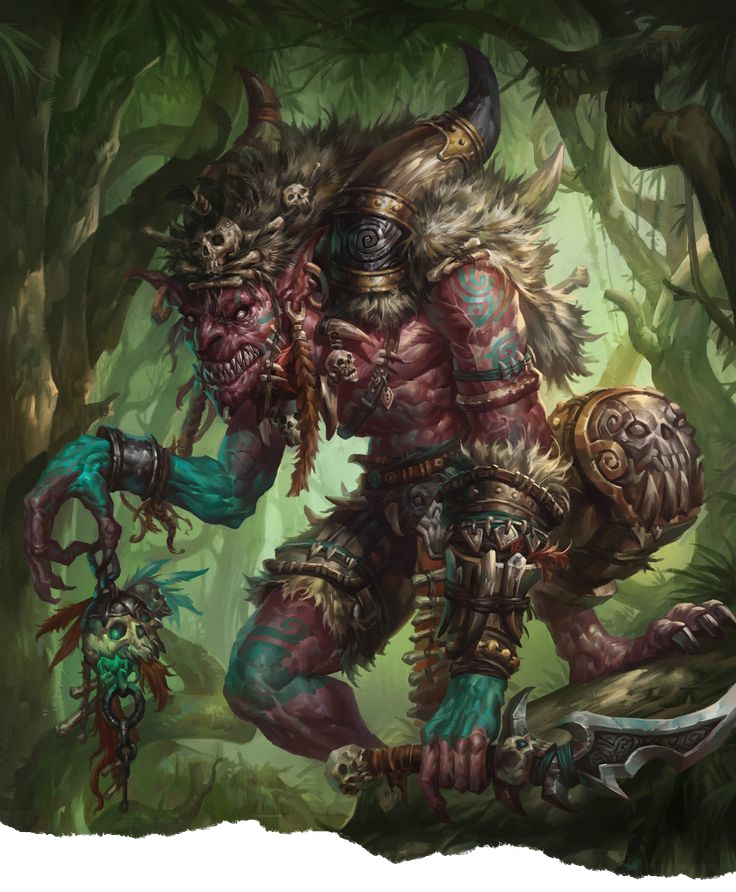
\includegraphics[scale=3.6]{media/chaman-hobgoblin.png}};
\end{tikzpicture}


% Monster stat block
\begin{DndMonster}[float*=b,width=\textwidth + 8pt]{Gheed}
    \begin{multicols}{2}
        \DndMonsterType{Chamán hobgoblin, legal malvado}

    % If you want to use commas in the key values, enclose the values in braces.
    \DndMonsterBasics[
	armor-class = {12 con \emph{armadura de cuero}},
        hit-points  = {\DndDice{3d8 + 3}},
        speed       = {30 ft},
      ]

    \DndMonsterAbilityScores[
        str = 13,
        dex = 14,
        con = 13,
        int = 10,
        wis = 10,
        cha = 8,
      ]

    \DndMonsterDetails[
        %saving-throws = {Str +0, Dex +0, Con +0, Int +0, Wis +0, Cha +0},
        %skills = {Acrobatics +0, Animal Handling +0, Arcana +0, Athletics +0, Deception +0, History +0, Insight +0, Intimidation +0, Investigation +0, Medicine +0, Nature +0, Perception +0, Performance +0, Persuasion +0, Religion +0, Sleight of Hand +0, Stealth +0, Survival +0},
        %damage-vulnerabilities = {cold},
        %damage-resistances = {bludgeoning, piercing, and slashing from nonmagical attacks},
        %damage-immunities = {poison},
        %condition-immunities = {poisoned},
        senses = {visión en la oscuridad 60 pies, percepción pasiva 10},
        languages = {común, goblin},
        challenge = 3,
      ]
    % Traits
    \DndMonsterAction{Innate Spellcasting}
    Foo's spellcasting ability is Charisma (spell save DC 12, +4 to hit with spell attacks). It can innately cast the following spells, requiring no material components:
    \begin{DndMonsterSpells}
      \DndInnateSpellLevel{misty step}
      \DndInnateSpellLevel[3]{fog cloud, rope trick}
      \DndInnateSpellLevel[1]{identify}
    \end{DndMonsterSpells}

    \DndMonsterAction{Spellcasting}
    Foo is a 2nd-level spellcaster. Its spellcasting ability is Charisma (spell save DC 12, +4 to hit with spell attacks). It has the following sorcerer spells prepared:
    \begin{DndMonsterSpells}
      \DndMonsterSpellLevel{blade ward, fire bolt, light, shocking grasp}
      \DndMonsterSpellLevel[1][3]{burning hands, mage armor, shield}
    \end{DndMonsterSpells}

    \DndMonsterSection{Actions}
    \DndMonsterAction{Multiattack}
    The foo makes two melee attacks.

    %Default values are shown commented out
    \DndMonsterAttack[
      name=Dagger,
      %distance=both, % valid options are in the set {both,melee,ranged},
      %type=weapon, %valid options are in the set {weapon,spell}
      mod=+3,
      %reach=5,
      %range=20/60,
      %targets=one target,
      dmg=\DndDice{1d4+1},
      dmg-type=piercing,
      %plus-dmg=,
      %plus-dmg-type=,
      %or-dmg=,
      %or-dmg-when=,
      %extra=,
    ]

    %\DndMonsterMelee calls \DndMonsterAttack with the melee option
    \DndMonsterMelee[
      name=Flame Tongue Longsword,
      mod=+3,
      %reach=5,
      %targets=one target,
      dmg=\DndDice{1d8+1},
      dmg-type=slashing,
      plus-dmg=\DndDice{2d6},
      plus-dmg-type=fire,
      or-dmg=\DndDice{1d10+1},
      or-dmg-when=if used with two hands,
      %extra=,
    ]

    %\DndMonsterRanged calls \DndMonsterAttack with the ranged option
    \DndMonsterRanged[
      name=Assassin's Light Crossbow,
      mod=+1,
      range=80/320,
      dmg=\DndDice{1d8},
      dmg-type=piercing,
      %plus-dmg=,
      %plus-dmg-type=,
      %or-dmg=,
      %or-dmg-when=,
      extra={, and the target must make a DC 15 Constitution saving throw, taking 24 (7d6) poison damage on a failed save, or half as much damage on a successful one}
    ]

    % Legendary Actions
    \DndMonsterSection{Legendary Actions}
    The foo can take 3 legendary actions, choosing from the options below. Only one legendary action option can be used at a time and only at the end of another creature's turn. The foo regains spent legendary actions at the start of its turn.

    \begin{DndMonsterLegendaryActions}
      \DndMonsterLegendaryAction{Move}{The foo moves up to its speed.}
      \DndMonsterLegendaryAction{Dagger Attack}{The foo makes a dagger attack.}
      \DndMonsterLegendaryAction{Create Contract (Costs 3 Actions)}{The foo presents a contract in a language it knows and waves it in the face of a creature within 10 feet. The creature must make a DC 10 Intelligence saving throw. On a failure, the creature is incapacitated until the start of the foo's next turn. A creature who cannot read the language in which the contract is written has advantage on this saving throw.}
    \end{DndMonsterLegendaryActions}
  \end{multicols}
\end{DndMonster}



\end{document}
